% Compiles the measurement chapter on its own: pdflatex measurements_standalone && bibtex measurements_standalone
% && pdflatex measurements_standalone && pdflatex measurements_standalone. In the thesis, % Measurement chapter: draft. Source of truth: results/box/*/REPORT.md (one per test), with the raw
% data, the analysis scripts and the predictions registered before each run.
% Needs: booktabs, graphicx, cleveref; refers to ch:theory (\chapref) for the model's assumptions.
\providecommand{\chapref}[2]{\cref{#1}}

\chapter{Measurements on a test machine}
\label{ch:measure}

The theory of \chapref{ch:theory}{Chapter~4} takes a few numbers per function as given: how long a
snapshot restore takes, how much warm-up is left after it, how much parallel restores slow each
other down, and how a start-up responds to CPU. The simulator used estimates for all of them. This
chapter measures them on real hardware, and answers two questions raised in review: whether a
snapshot mechanism is worth its cost against what the JDK itself now offers, and whether the
premise of the CPU plan holds.

\section{Method}
\label{sec:m-method}

\paragraph{Machine.} A virtual machine with 8 Intel Xeon Gold 6248R cores (2 sockets, one thread
per core), 31\,GB of memory, Ubuntu 24.04 with Linux 6.8, cgroup v2, no CPU steal time (checked
with \texttt{vmstat}), on VMware. Software: Docker 29.8, CRIU 4.2.1, the Zulu CRaC build of
OpenJDK 21.0.12, and OpenJDK 25.0.4. CPU quotas are set with the cgroup \texttt{cpu.max} file;
CPU-seconds and throttled periods are read from \texttt{cpu.stat}.

\paragraph{Workload.} A Spring Boot function (web starter, Jackson, Hibernate Validator) whose
handler deserialises, validates, aggregates and serialises a list of 400 orders; the service is
called directly, so the measurement is of framework start-up and JIT warm-up, not of socket
handling. Every run uses the same serving shape: \texttt{-XX:ActiveProcessorCount=1}, the serial
collector, a 256--512\,MB heap.

\paragraph{Snapshots.} Snapshots are taken with CRaC (Coordinated Restore at Checkpoint): the
function calls the checkpoint itself after $K$ warm-up requests (depth $K$), and a restore resumes
it at that point. CRaC has two engines. The Zulu build checkpoints with Azul's \emph{Warp} engine
unless told otherwise; CRIU is selected with \texttt{-XX:CRaCEngine=criu}. Most measurements below
used Warp; \cref{sec:m-engines} compares the two engines directly and shows that the conclusions
hold for CRIU.

\paragraph{Metrics.} \emph{Time to first response} (TTFR): from the launch of the process, or of
the restore, to the moment the first request's response is complete, measured outside the process
(the function prints the wall-clock time of its first response). After the first response every
run serves the same 200 requests. $C$ is the steady latency (median of requests 150--200 of the
most warmed process); the \emph{residual warm-up} is $R = \sum_i \max(0, \ell_i - C)$ over the first
request and the 200 after it, where $\ell_i$ is the latency of request $i$; for a cold start this
is the warm-up $B$.

\paragraph{Rules.} Every test followed the same rules. Its prediction was written and committed
before the run. It has a control whose answer is known in advance, run first. Each cell has
$n \ge 20$ repetitions in random order. Raw data has one row per run and is never edited. Medians
are reported with 95\% bootstrap confidence intervals (10{,}000 resamples). A falsified
prediction is reported as a result. \Cref{tab:m-predictions} lists every prediction and its outcome.

\section{Is a snapshot worth it?}
\label{sec:m-aot}

JDK~24 and~25 ship a competitor that needs no snapshot: the ahead-of-time cache of Project
Leyden~\cite{jep483,jep514,jep515}. A training run records the classes it loaded and linked, and
the profiles of the methods it ran; later starts reuse them. It needs no special privileges and
cannot clone secrets. If it came close to a snapshot restore, a snapshot mechanism would not be
worth its operational cost. The registered decision rule: a snapshot is justified if it reaches the
first response at least $3\times$ sooner than the AOT cache trained with the same requests, at both
CPU levels.

\begin{table}[htbp]
\centering
\caption{Start modes of the same function: time to first response (median, $n = 20$) and CPU per
start. The AOT cache and the restore at depth 50 saw the same 50 training requests.}
\label{tab:m-aot}
\small
\begin{tabular}{@{}lrrr@{}}
\toprule
start mode & 0.25 vCPU & 1 vCPU & CPU-s \\
\midrule
cold start, JDK 21 / JDK 25 & 16.9 / 17.6\,s & 3.97 / 4.08\,s & 5.4--5.7 \\
JIT capped at C1 (\texttt{-XX:TieredStopAtLevel=1}) & 9.8\,s & 2.32\,s & 3.0 \\
JDK 25 AOT cache, trained with start-up only & 9.5\,s & 2.26\,s & 3.6--3.7 \\
JDK 25 AOT cache, trained with 50 requests & 8.7\,s & 2.05\,s & 3.0--3.3 \\
snapshot restore after start-up ($K = 0$, Warp) & 2.09\,s & 0.50\,s & 2.0 \\
snapshot restore at $K = 50$, Warp & \textbf{0.29\,s} & \textbf{0.08\,s} & 1.2 \\
snapshot restore at $K = 50$, CRIU & \textbf{0.38\,s} & \textbf{0.08\,s} & 1.0 \\
\bottomrule
\end{tabular}
\end{table}

\Cref{tab:m-aot} shows the result. The AOT cache roughly halves a cold start ($0.54$--$0.55\times$),
as published for Spring applications. A snapshot at depth 50 answers its first request
\textbf{25--30$\times$ sooner} than the AOT cache with the same training (95\% confidence
intervals of the ratio: $[29.2, 33.1]$ at 0.25\,vCPU, $[23.3, 31.7]$ at 1\,vCPU; with the CRIU engine
$\approx 23$--$24\times$), and uses about $2.5\times$ less CPU per start. Even the snapshot point
of current restore-on-demand systems ($K = 0$) is $4.5\times$ ahead. The control passed: cold
starts on JDK~21 and~25 differ by 3--4\%, so the comparison is not an artefact of the JDK version.

One prediction failed. After a depth-50 restore, the residual warm-up over the next 200 requests
is \emph{not} smaller than after the AOT cache (720 vs 652\,ms at 1\,vCPU, overlapping intervals).
A snapshot's advantage is the first response; the JIT still has work to do afterwards
(\cref{sec:m-depth}).

\section{The two engines}
\label{sec:m-engines}

\begin{table}[htbp]
\centering
\caption{Warp vs CRIU on the same function (time to first response, median [95\% CI], $n = 20$).}
\label{tab:m-engines}
\small
\begin{tabular}{@{}rrrrr@{}}
\toprule
vCPU & $K$ & Warp & CRIU & difference \\
\midrule
1 & 0 & 474 [463, 483]\,ms & 492 [482, 502]\,ms & $+18$\,ms \\
1 & 50 & 67 [61, 72]\,ms & 84 [80, 91]\,ms & $+17$\,ms \\
0.25 & 0 & 1986 [1967, 2035]\,ms & 2076 [2066, 2131]\,ms & $+90$\,ms \\
0.25 & 50 & 284 [280, 291]\,ms & 375 [301, 385]\,ms & $+91$\,ms \\
\bottomrule
\end{tabular}
\end{table}

All 160 restores and 16 checkpoints succeeded with both engines. CRIU is 17--91\,ms slower per
restore (\cref{tab:m-engines}), with the same CPU-seconds and similar image sizes (78--98 vs
79--93\,MB). The prediction, ``a few hundred milliseconds slower'', was falsified in CRIU's
favour. The first request after the restore takes the same time with either engine, so the
engines differ only in the restore itself. The design does not depend on the engine.

\section{Parallel restores}
\label{sec:m-parallel}

Look-ahead restores several stages at once. \Cref{cor:contention} of \chapref{ch:theory}{Chapter~4}
bounds the gain by $(1 - \beta)$, where $\beta$ measures how much $N$ simultaneous restores slow
the slowest one: $\beta(N) = (r_{\max}(N)/r(1) - 1)/(N - 1)$; $\beta = 1$ means the restores
run one after another.

The snapshot (Warp, $K = 50$) was restored $N \in \{1, 2, 4, 8\}$ times at once, each copy in its
own Docker container with its own CPU quota, 20 repetitions, about 2{,}400 restores in total,
none failed. Through \texttt{docker run}, $\beta(4) = 0.21$ $[0.17, 0.27]$ at 0.25\,vCPU and
$0.53$ $[0.35, 0.67]$ at 1\,vCPU. A control that starts the same number of containers running an
empty command slows down exactly as much: Docker creates containers one after another, about
250\,ms each~\cite{forkroad2025}. Restoring into containers created beforehand (as OpenWhisk's
prewarmed ``stem cell'' containers are) removes it:

\begin{center}
\small
\begin{tabular}{@{}lrrrrr@{}}
\toprule
restore into an existing container & $N = 1$ & 2 & 4 & 8 & $\beta(4)$ [95\% CI] \\
\midrule
0.25\,vCPU & 380\,ms & 418 & 429 & 456 & 0.04 [0.01, 0.08] \\
1\,vCPU & 101\,ms & 106 & 122 & 201 & 0.07 [0.03, 0.09] \\
\bottomrule
\end{tabular}
\end{center}

The restores themselves barely compete: eight at once cost 76--100\,ms more than one. The
serial control (each copy started when the previous one answered) gave $\beta = 1.04$--$1.14$ at
0.25\,vCPU, as it must, but 1.23--1.63 at 1\,vCPU, because each copy's remaining work overlapped
the next copy's start; the result for pre-created containers does not depend on this control.
\textbf{Design consequence:} the platform should restore into existing containers, not create a
container per restore.

\section{The function's profile against snapshot depth}
\label{sec:m-depth}

Snapshots were taken after $K \in \{0, 1, 5, 20, 50, 100, 200\}$ requests (4 images each, built at
1\,vCPU) and restored at 0.25, 0.5, 1, 2 and 4\,vCPU, 20 times each, interleaved with cold starts
and with processes that were never checkpointed: 1{,}280 runs, none failed.

\begin{table}[htbp]
\centering
\caption{The profile (Warp; ms, median of 20). TTFR / $R$ for restores; $B$ for cold starts.}
\label{tab:m-profile}
\small
\begin{tabular}{@{}rrrrrr@{}}
\toprule
vCPU & cold TTFR / $B$ & $K = 0$ & $K = 50$ & $K = 200$ & never checkpointed, $K = 200$: $R$ \\
\midrule
0.25 & 16\,551 / 5\,759 & 2\,675 / 7\,310 & 380 / 3\,570 & 875 / 2\,313 & 1\,563 \\
0.5 & 7\,981 / 3\,084 & 1\,025 / 3\,590 & 163 / 1\,656 & 161 / 1\,105 & 811 \\
1 & 3\,968 / 1\,271 & 758 / 1\,606 & 181 / 720 & 297 / 453 & 342 \\
2 & 1\,988 / 628 & 267 / 753 & 61 / 280 & 60 / 165 & 93 \\
4 & 1\,798 / 561 & 248 / 577 & 59 / 229 & 58 / 112 & 69 \\
\bottomrule
\end{tabular}
\end{table}

\paragraph{Image size} is flat in $K$: 82--88\,MB at every depth (the earlier cost analysis
assumed 90\,MB). \paragraph{Restore time} is flat in $K$ for $K \ge 5$: about 60\,ms at 2 and 4\,vCPU
and 67--84\,ms at 1\,vCPU (\cref{tab:m-engines}). The theory's examples used 650\,ms; a deep
restore is an order of magnitude cheaper. \paragraph{Residual warm-up} falls with depth and does
not level off by $K = 200$ (at 1\,vCPU: 1\,606, 720, 453\,ms at $K = 0$, 50, 200); the predicted
63\,ms at $K = 50$ (from a lighter function) was off by $11\times$. The JIT is still compiling at
$K = 200$: compile time at the checkpoint grows from 4.5 to 6.7\,s and the code cache from 7.6 to
9.4\,MB between $K = 0$ and 200. \Cref{prop:depth}'s stopping rule (stop when compilation stops)
therefore did not trigger within 200 requests on this function.

\paragraph{An anomaly.} At 0.25 and 1\,vCPU, deep restores in this experiment were bimodal: at
1\,vCPU and $K = 50$, ten runs took 61--88\,ms and ten 274--386\,ms. The same images restored in
59\,ms when the runs were not interleaved with cold starts, and the dedicated engine test measured
67--84\,ms unimodally. It is not eviction from the page cache (the cgroup recorded no refaults), not
disk (a restore from disk takes about 505\,ms), and not one image (all four show both modes). Its
cause is open; the restore times quoted above are taken from the experiments without it.

\paragraph{Disk.} With the page cache dropped first, a depth-50 restore takes 505\,ms at 1\,vCPU and
1\,094\,ms at 0.25\,vCPU, against 67 and 284\,ms from memory: reading an 88\,MB image costs more
than the restore. An invoker should keep its images in memory.

\section{Warm-up lost to the checkpoint, and re-warming}
\label{sec:m-rewarm}

A restored process has more warm-up left than the same process never checkpointed. The loss
$L(K) = R_{\text{restored}} - R_{\text{never checkpointed}}$ at $K = 50$ is 955\,ms at 0.25\,vCPU,
163\,ms at 1\,vCPU and indistinguishable from zero at 2--4\,vCPU (several intervals include zero;
$K = 200$ is clearly positive up to 2\,vCPU). The loss is larger where CPU is scarce, as predicted.
A restored sandbox that serves 50 more test requests while it waits for its input
(\emph{re-warming}) ends with \emph{less} residual than the never-checkpointed process (1\,762 vs
2\,615\,ms at 0.25\,vCPU; 337 vs 556\,ms at 1\,vCPU): re-warming does not just recover the loss, it
deepens the snapshot. It costs 1.3\,s of waiting time at 0.25\,vCPU and 0.3\,s at 1\,vCPU.

\section{CPU during start-up}
\label{sec:m-cpu}

The CPU plan (\cref{sec:th-cpu}) rests on assumption B1 (\cref{tab:cpu-assumptions}): a start-up
finishes in proportion to the CPU it gets, at the same CPU-seconds.

\begin{table}[htbp]
\centering
\caption{Speed-up of the time to first response relative to 0.25\,vCPU, and CPU-seconds per start
(median of 20).}
\label{tab:m-speedup}
\small
\begin{tabular}{@{}lrrrrr@{}}
\toprule
mode & 0.5 & 1 & 2 & 4\,vCPU & CPU-s, 0.25 $\to$ 4\,vCPU \\
\midrule
cold start & $2.07\times$ & $4.17\times$ & $8.32\times$ & $9.2\times$ & $5.40 \to 5.16$ \\
restore, $K = 0$ & $2.61\times$ & $3.53\times$ & $10.0\times$ & $10.8\times$ & $2.11 \to 1.85$ \\
restore, $K = 50$ (engine test) & & $4.2$--$4.5\times$ & & & $1.1 \to 1.0$ \\
\bottomrule
\end{tabular}
\end{table}

\paragraph{B1 holds, beyond one core} (\cref{tab:m-speedup}). A cold JVM start is $4.2\times$ faster
with four times the CPU and $8.3\times$ faster with eight times, using the same CPU-seconds
(within 6\%) at every quota. It levels off only past 2\,vCPU. A JVM told it has one processor still
uses about two cores while it starts (collector, compiler and class-loading threads). The model's
cap of one core per start-up is therefore too low; about two cores is right for this runtime.

\paragraph{Boosting only while starting.} A start-up was given 1 or 2\,vCPU and lowered to
0.25\,vCPU the moment its first response was out (the change took effect within 1.4--4.8\,ms).
Boosting costs no extra CPU. For a deep restore the following requests were as fast as without the
boost (1.71 vs 1.68\,ms). For a cold start or a restore at $K = 0$ they were 17--52\% slower: the
boost brought the first response forward, so less compilation had happened by then, and the rest
of the warm-up moved into the following requests. \textbf{The boost buys the first response, not
the warm-up}; it should last until the warm-up is done.

\paragraph{One core, several start-ups.} Two or four depth-50 restores shared one core, either
split equally or one at a time at the full core (\cref{prop:cpu-onecore}). One at a time made them
ready 19--27\% sooner on average (4 restores: 203 vs 279\,ms) and the first one 1.9--3.6$\times$
sooner, at an 8--12\% later last one, as the proposition predicts.

\paragraph{The cliff.} \Cref{fig:m-cliff} shows the time to first response plus the residual
warm-up against the quota. A cold start's warm-up grows $10.3\times$ from 4 to 0.25\,vCPU (an
earlier measurement on a heavier warm-up gave 13--35$\times$). The prediction that deep snapshots
flatten this cliff was falsified as a ratio: the deeper the snapshot, the steeper the relative
cliff ($12.7\times$ at $K = 0$, $20.6\times$ at $K = 200$), because at 4\,vCPU a deep restore leaves
almost nothing. In absolute time it holds: a deep snapshot saves 19.1\,s per start at 0.25\,vCPU
and 2.2\,s at 4\,vCPU. Snapshots save the most exactly where serverless functions run.

\begin{figure}[htbp]
\centering
\IfFileExists{../figures/fig9_cliff.pdf}{\includegraphics[width=\textwidth]{fig9_cliff}}%
  {\fbox{\parbox{0.9\textwidth}{\centering figures/fig9\_cliff.pdf not rendered yet:
  run \texttt{python3 figures/make\_figures.py}}}}
\caption{Time to first response plus residual warm-up against the CPU quota, for a cold start, a
snapshot after start-up ($K = 0$) and a deep snapshot ($K = 200$); median of 20 runs per point,
logarithmic axes.}
\label{fig:m-cliff}
\end{figure}

\section{Safety: what restored copies share}
\label{sec:m-uniq}

Copies restored from one image start with the same memory~\cite{brooker2021}. Ten copies were
restored from one image and each reported hashes of values it had created at start-up. Without
reset hooks, a \texttt{java.util.Random}, a secret token generated at start-up (even from a
\texttt{SecureRandom}) and \texttt{Math.random()} returned the same value in all ten copies; the
JDK's own \texttt{SecureRandom} and \texttt{UUID} sources were re-seeded on restore and differed.
A CRaC resource hook that re-seeds the \texttt{Random} and regenerates the token fixed those two
(ten distinct values), but \textbf{not \texttt{Math.random()}}, whose generator is private to the
JDK and has no re-seed interface. A snapshot builder must therefore either refuse functions that
call \texttt{Math.random()} before the checkpoint, or reset its generator by reflection; this is
one concrete reason why not every function is safe to snapshot.

\section{What the measurements change}
\label{sec:m-changes}

\begin{itemize}
\item \textbf{The model's inputs.} Restore time $r$: 74--84\,ms at 1\,vCPU and 282--375\,ms at
      0.25\,vCPU for a deep snapshot (was 650\,ms). Contention $\beta \approx 0.05$ into existing
      containers (was an assumption). Residual warm-up after a restore: 720\,ms over 200 requests
      at $K = 50$, 1\,vCPU (was 63\,ms). Start-up cap: about two cores (was one).
\item \textbf{The weight shifts from timing to depth and CPU.} With $r \approx 80$\,ms, restoring
      ahead hides about 80\,ms per stage at 1\,vCPU and about 300\,ms at 0.25\,vCPU. The residual
      warm-up and the CPU a start-up gets now matter more than when it starts.
\item \textbf{The design.} Restore into existing containers; keep images in memory; boost a
      start-up until its warm-up is done; keep re-warming; choose the depth from the residual
      curve rather than from a compile counter that has not levelled off; exclude or patch
      functions that use \texttt{Math.random()} before the checkpoint.
\end{itemize}

\begin{table}[htbp]
\centering
\caption{Registered predictions and outcomes.}
\label{tab:m-predictions}
\small
\begin{tabular}{@{}p{0.5\textwidth}p{0.42\textwidth}@{}}
\toprule
prediction & outcome \\
\midrule
a deep snapshot reaches the first response $\ge 5\times$ sooner than the AOT cache & confirmed, 25--30$\times$ \\
residual warm-up after a deep restore $\ll$ after the AOT cache & falsified: similar \\
CRIU a few hundred ms slower than Warp & falsified: 17--91\,ms \\
$\beta < 0.3$ for $N \le 4$ & confirmed into existing containers; through \texttt{docker run} only at 0.25\,vCPU \\
Docker's own part of $\beta$: 0.1--0.3 & falsified: 0.6--0.8 \\
image size flat in $K$ & confirmed, 82--88\,MB \\
residual warm-up $\approx 63$\,ms at $K = 50$, levelling off & falsified: 720\,ms, still falling at $K = 200$ \\
restore from disk $< 50$\,ms slower than from memory & falsified: 440--810\,ms \\
$L(K) > 0$, larger at low CPU; re-warming recovers $\ge 30\%$ & confirmed; recovers more than all of it \\
reset hooks make every value distinct & falsified for \texttt{Math.random()} \\
cold warm-up cliff 13--35$\times$ & falsified in size: $10.3\times$ \\
deep snapshots flatten the cliff (ratio $< 5\times$) & falsified as a ratio ($20.6\times$); holds in absolute time \\
start-up $\approx 4\times$ faster from 0.25 to 1\,vCPU at the same CPU-seconds & confirmed ($3.5$--$4.5\times$); continues to 2 cores \\
boosted start-ups serve later requests as fast & confirmed for deep restores; falsified for cold starts and $K = 0$ \\
\bottomrule
\end{tabular}
\end{table}

\section{Threats to validity}
\label{sec:m-threats}

\begin{itemize}
\item \textbf{One function.} All numbers are for one Spring Boot function. The residual warm-up and
      the depth at which it levels off depend on the function; the qualitative results
      (snapshot vs AOT cache, contention into existing containers, the shape of the speed-up)
      are the ones to generalise, and the next experiments add Python and ML stages.
\item \textbf{A virtual machine.} The host is VMware with no measured steal time; the disk is
      virtual, so the disk tier's cost is specific to it.
\item \textbf{Memory was not measured.} The cgroup's memory counter included the page cache it
      had accumulated, so the processes' own memory is unknown; image sizes are reported instead.
\item \textbf{The bimodal restores} (\cref{sec:m-depth}) are unexplained.
\item \textbf{Privileges.} Containers ran with \texttt{--privileged}; the minimal capability set,
      and CRIU inside pre-created containers, are left to the OpenWhisk integration.
\end{itemize}

% from the department's template instead (thesis/README.md).
\documentclass[11pt,a4paper]{report}
\usepackage[T1]{fontenc}
\usepackage{lmodern}
\usepackage[margin=2.5cm]{geometry}
\usepackage{amsmath,amssymb,amsthm,mathtools}
\usepackage{enumitem,booktabs,graphicx,xcolor,tikz}
\usepackage{algorithm}
\usepackage[noend]{algpseudocode}
\usepackage{microtype}
\usepackage{xr-hyper}
\externaldocument{theory_standalone}  % labels of the theory chapter (build it first)
\usepackage[hidelinks]{hyperref}
\usepackage[capitalise,noabbrev]{cleveref}
\graphicspath{{../figures/}}

\theoremstyle{plain}
\newtheorem{theorem}{Theorem}[chapter]
\newtheorem{corollary}[theorem]{Corollary}
\newtheorem{lemma}[theorem]{Lemma}
\newtheorem{proposition}[theorem]{Proposition}
\theoremstyle{definition}
\newtheorem{definition}[theorem]{Definition}
\newtheorem{example}[theorem]{Example}

\newcommand{\chapref}[2]{#2}

\title{Measurements on a test machine\\[4pt]\large Measurement chapter, draft}
\author{MSc thesis, Amirkabir University of Technology}
\date{\today}

\begin{document}
\maketitle
\setcounter{chapter}{2}
% Measurement chapter: draft. Source of truth: results/box/*/REPORT.md (one per test), with the raw
% data, the analysis scripts and the predictions registered before each run.
% Needs: booktabs, graphicx, cleveref; refers to ch:theory (\chapref) for the model's assumptions.
\providecommand{\chapref}[2]{\cref{#1}}

\chapter{Measurements on a test machine}
\label{ch:measure}

The theory of \chapref{ch:theory}{Chapter~4} takes a few numbers per function as given: how long a
snapshot restore takes, how much warm-up is left after it, how much parallel restores slow each
other down, and how a start-up responds to CPU. The simulator used estimates for all of them. This
chapter measures them on real hardware, and answers two questions raised in review: whether a
snapshot mechanism is worth its cost against what the JDK itself now offers, and whether the
premise of the CPU plan holds.

\section{Method}
\label{sec:m-method}

\paragraph{Machine.} A virtual machine with 8 Intel Xeon Gold 6248R cores (2 sockets, one thread
per core), 31\,GB of memory, Ubuntu 24.04 with Linux 6.8, cgroup v2, no CPU steal time (checked
with \texttt{vmstat}), on VMware. Software: Docker 29.8, CRIU 4.2.1, the Zulu CRaC build of
OpenJDK 21.0.12, and OpenJDK 25.0.4. CPU quotas are set with the cgroup \texttt{cpu.max} file;
CPU-seconds and throttled periods are read from \texttt{cpu.stat}.

\paragraph{Workload.} A Spring Boot function (web starter, Jackson, Hibernate Validator) whose
handler deserialises, validates, aggregates and serialises a list of 400 orders; the service is
called directly, so the measurement is of framework start-up and JIT warm-up, not of socket
handling. Every run uses the same serving shape: \texttt{-XX:ActiveProcessorCount=1}, the serial
collector, a 256--512\,MB heap.

\paragraph{Snapshots.} Snapshots are taken with CRaC (Coordinated Restore at Checkpoint): the
function calls the checkpoint itself after $K$ warm-up requests (depth $K$), and a restore resumes
it at that point. CRaC has two engines. The Zulu build checkpoints with Azul's \emph{Warp} engine
unless told otherwise; CRIU is selected with \texttt{-XX:CRaCEngine=criu}. Most measurements below
used Warp; \cref{sec:m-engines} compares the two engines directly and shows that the conclusions
hold for CRIU.

\paragraph{Metrics.} \emph{Time to first response} (TTFR): from the launch of the process, or of
the restore, to the moment the first request's response is complete, measured outside the process
(the function prints the wall-clock time of its first response). After the first response every
run serves the same 200 requests. $C$ is the steady latency (median of requests 150--200 of the
most warmed process); the \emph{residual warm-up} is $R = \sum_i \max(0, \ell_i - C)$ over the first
request and the 200 after it, where $\ell_i$ is the latency of request $i$; for a cold start this
is the warm-up $B$.

\paragraph{Rules.} Every test followed the same rules. Its prediction was written and committed
before the run. It has a control whose answer is known in advance, run first. Each cell has
$n \ge 20$ repetitions in random order. Raw data has one row per run and is never edited. Medians
are reported with 95\% bootstrap confidence intervals (10{,}000 resamples). A falsified
prediction is reported as a result. \Cref{tab:m-predictions} lists every prediction and its outcome.

\section{Is a snapshot worth it?}
\label{sec:m-aot}

JDK~24 and~25 ship a competitor that needs no snapshot: the ahead-of-time cache of Project
Leyden~\cite{jep483,jep514,jep515}. A training run records the classes it loaded and linked, and
the profiles of the methods it ran; later starts reuse them. It needs no special privileges and
cannot clone secrets. If it came close to a snapshot restore, a snapshot mechanism would not be
worth its operational cost. The registered decision rule: a snapshot is justified if it reaches the
first response at least $3\times$ sooner than the AOT cache trained with the same requests, at both
CPU levels.

\begin{table}[htbp]
\centering
\caption{Start modes of the same function: time to first response (median, $n = 20$) and CPU per
start. The AOT cache and the restore at depth 50 saw the same 50 training requests.}
\label{tab:m-aot}
\small
\begin{tabular}{@{}lrrr@{}}
\toprule
start mode & 0.25 vCPU & 1 vCPU & CPU-s \\
\midrule
cold start, JDK 21 / JDK 25 & 16.9 / 17.6\,s & 3.97 / 4.08\,s & 5.4--5.7 \\
JIT capped at C1 (\texttt{-XX:TieredStopAtLevel=1}) & 9.8\,s & 2.32\,s & 3.0 \\
JDK 25 AOT cache, trained with start-up only & 9.5\,s & 2.26\,s & 3.6--3.7 \\
JDK 25 AOT cache, trained with 50 requests & 8.7\,s & 2.05\,s & 3.0--3.3 \\
snapshot restore after start-up ($K = 0$, Warp) & 2.09\,s & 0.50\,s & 2.0 \\
snapshot restore at $K = 50$, Warp & \textbf{0.29\,s} & \textbf{0.08\,s} & 1.2 \\
snapshot restore at $K = 50$, CRIU & \textbf{0.38\,s} & \textbf{0.08\,s} & 1.0 \\
\bottomrule
\end{tabular}
\end{table}

\Cref{tab:m-aot} shows the result. The AOT cache roughly halves a cold start ($0.54$--$0.55\times$),
as published for Spring applications. A snapshot at depth 50 answers its first request
\textbf{25--30$\times$ sooner} than the AOT cache with the same training (95\% confidence
intervals of the ratio: $[29.2, 33.1]$ at 0.25\,vCPU, $[23.3, 31.7]$ at 1\,vCPU; with the CRIU engine
$\approx 23$--$24\times$), and uses about $2.5\times$ less CPU per start. Even the snapshot point
of current restore-on-demand systems ($K = 0$) is $4.5\times$ ahead. The control passed: cold
starts on JDK~21 and~25 differ by 3--4\%, so the comparison is not an artefact of the JDK version.

One prediction failed. After a depth-50 restore, the residual warm-up over the next 200 requests
is \emph{not} smaller than after the AOT cache (720 vs 652\,ms at 1\,vCPU, overlapping intervals).
A snapshot's advantage is the first response; the JIT still has work to do afterwards
(\cref{sec:m-depth}).

\section{The two engines}
\label{sec:m-engines}

\begin{table}[htbp]
\centering
\caption{Warp vs CRIU on the same function (time to first response, median [95\% CI], $n = 20$).}
\label{tab:m-engines}
\small
\begin{tabular}{@{}rrrrr@{}}
\toprule
vCPU & $K$ & Warp & CRIU & difference \\
\midrule
1 & 0 & 474 [463, 483]\,ms & 492 [482, 502]\,ms & $+18$\,ms \\
1 & 50 & 67 [61, 72]\,ms & 84 [80, 91]\,ms & $+17$\,ms \\
0.25 & 0 & 1986 [1967, 2035]\,ms & 2076 [2066, 2131]\,ms & $+90$\,ms \\
0.25 & 50 & 284 [280, 291]\,ms & 375 [301, 385]\,ms & $+91$\,ms \\
\bottomrule
\end{tabular}
\end{table}

All 160 restores and 16 checkpoints succeeded with both engines. CRIU is 17--91\,ms slower per
restore (\cref{tab:m-engines}), with the same CPU-seconds and similar image sizes (78--98 vs
79--93\,MB). The prediction, ``a few hundred milliseconds slower'', was falsified in CRIU's
favour. The first request after the restore takes the same time with either engine, so the
engines differ only in the restore itself. The design does not depend on the engine.

\section{Parallel restores}
\label{sec:m-parallel}

Look-ahead restores several stages at once. \Cref{cor:contention} of \chapref{ch:theory}{Chapter~4}
bounds the gain by $(1 - \beta)$, where $\beta$ measures how much $N$ simultaneous restores slow
the slowest one: $\beta(N) = (r_{\max}(N)/r(1) - 1)/(N - 1)$; $\beta = 1$ means the restores
run one after another.

The snapshot (Warp, $K = 50$) was restored $N \in \{1, 2, 4, 8\}$ times at once, each copy in its
own Docker container with its own CPU quota, 20 repetitions, about 2{,}400 restores in total,
none failed. Through \texttt{docker run}, $\beta(4) = 0.21$ $[0.17, 0.27]$ at 0.25\,vCPU and
$0.53$ $[0.35, 0.67]$ at 1\,vCPU. A control that starts the same number of containers running an
empty command slows down exactly as much: Docker creates containers one after another, about
250\,ms each~\cite{forkroad2025}. Restoring into containers created beforehand (as OpenWhisk's
prewarmed ``stem cell'' containers are) removes it:

\begin{center}
\small
\begin{tabular}{@{}lrrrrr@{}}
\toprule
restore into an existing container & $N = 1$ & 2 & 4 & 8 & $\beta(4)$ [95\% CI] \\
\midrule
0.25\,vCPU & 380\,ms & 418 & 429 & 456 & 0.04 [0.01, 0.08] \\
1\,vCPU & 101\,ms & 106 & 122 & 201 & 0.07 [0.03, 0.09] \\
\bottomrule
\end{tabular}
\end{center}

The restores themselves barely compete: eight at once cost 76--100\,ms more than one. The
serial control (each copy started when the previous one answered) gave $\beta = 1.04$--$1.14$ at
0.25\,vCPU, as it must, but 1.23--1.63 at 1\,vCPU, because each copy's remaining work overlapped
the next copy's start; the result for pre-created containers does not depend on this control.
\textbf{Design consequence:} the platform should restore into existing containers, not create a
container per restore.

\section{The function's profile against snapshot depth}
\label{sec:m-depth}

Snapshots were taken after $K \in \{0, 1, 5, 20, 50, 100, 200\}$ requests (4 images each, built at
1\,vCPU) and restored at 0.25, 0.5, 1, 2 and 4\,vCPU, 20 times each, interleaved with cold starts
and with processes that were never checkpointed: 1{,}280 runs, none failed.

\begin{table}[htbp]
\centering
\caption{The profile (Warp; ms, median of 20). TTFR / $R$ for restores; $B$ for cold starts.}
\label{tab:m-profile}
\small
\begin{tabular}{@{}rrrrrr@{}}
\toprule
vCPU & cold TTFR / $B$ & $K = 0$ & $K = 50$ & $K = 200$ & never checkpointed, $K = 200$: $R$ \\
\midrule
0.25 & 16\,551 / 5\,759 & 2\,675 / 7\,310 & 380 / 3\,570 & 875 / 2\,313 & 1\,563 \\
0.5 & 7\,981 / 3\,084 & 1\,025 / 3\,590 & 163 / 1\,656 & 161 / 1\,105 & 811 \\
1 & 3\,968 / 1\,271 & 758 / 1\,606 & 181 / 720 & 297 / 453 & 342 \\
2 & 1\,988 / 628 & 267 / 753 & 61 / 280 & 60 / 165 & 93 \\
4 & 1\,798 / 561 & 248 / 577 & 59 / 229 & 58 / 112 & 69 \\
\bottomrule
\end{tabular}
\end{table}

\paragraph{Image size} is flat in $K$: 82--88\,MB at every depth (the earlier cost analysis
assumed 90\,MB). \paragraph{Restore time} is flat in $K$ for $K \ge 5$: about 60\,ms at 2 and 4\,vCPU
and 67--84\,ms at 1\,vCPU (\cref{tab:m-engines}). The theory's examples used 650\,ms; a deep
restore is an order of magnitude cheaper. \paragraph{Residual warm-up} falls with depth and does
not level off by $K = 200$ (at 1\,vCPU: 1\,606, 720, 453\,ms at $K = 0$, 50, 200); the predicted
63\,ms at $K = 50$ (from a lighter function) was off by $11\times$. The JIT is still compiling at
$K = 200$: compile time at the checkpoint grows from 4.5 to 6.7\,s and the code cache from 7.6 to
9.4\,MB between $K = 0$ and 200. \Cref{prop:depth}'s stopping rule (stop when compilation stops)
therefore did not trigger within 200 requests on this function.

\paragraph{An anomaly.} At 0.25 and 1\,vCPU, deep restores in this experiment were bimodal: at
1\,vCPU and $K = 50$, ten runs took 61--88\,ms and ten 274--386\,ms. The same images restored in
59\,ms when the runs were not interleaved with cold starts, and the dedicated engine test measured
67--84\,ms unimodally. It is not eviction from the page cache (the cgroup recorded no refaults), not
disk (a restore from disk takes about 505\,ms), and not one image (all four show both modes). Its
cause is open; the restore times quoted above are taken from the experiments without it.

\paragraph{Disk.} With the page cache dropped first, a depth-50 restore takes 505\,ms at 1\,vCPU and
1\,094\,ms at 0.25\,vCPU, against 67 and 284\,ms from memory: reading an 88\,MB image costs more
than the restore. An invoker should keep its images in memory.

\section{Warm-up lost to the checkpoint, and re-warming}
\label{sec:m-rewarm}

A restored process has more warm-up left than the same process never checkpointed. The loss
$L(K) = R_{\text{restored}} - R_{\text{never checkpointed}}$ at $K = 50$ is 955\,ms at 0.25\,vCPU,
163\,ms at 1\,vCPU and indistinguishable from zero at 2--4\,vCPU (several intervals include zero;
$K = 200$ is clearly positive up to 2\,vCPU). The loss is larger where CPU is scarce, as predicted.
A restored sandbox that serves 50 more test requests while it waits for its input
(\emph{re-warming}) ends with \emph{less} residual than the never-checkpointed process (1\,762 vs
2\,615\,ms at 0.25\,vCPU; 337 vs 556\,ms at 1\,vCPU): re-warming does not just recover the loss, it
deepens the snapshot. It costs 1.3\,s of waiting time at 0.25\,vCPU and 0.3\,s at 1\,vCPU.

\section{CPU during start-up}
\label{sec:m-cpu}

The CPU plan (\cref{sec:th-cpu}) rests on assumption B1 (\cref{tab:cpu-assumptions}): a start-up
finishes in proportion to the CPU it gets, at the same CPU-seconds.

\begin{table}[htbp]
\centering
\caption{Speed-up of the time to first response relative to 0.25\,vCPU, and CPU-seconds per start
(median of 20).}
\label{tab:m-speedup}
\small
\begin{tabular}{@{}lrrrrr@{}}
\toprule
mode & 0.5 & 1 & 2 & 4\,vCPU & CPU-s, 0.25 $\to$ 4\,vCPU \\
\midrule
cold start & $2.07\times$ & $4.17\times$ & $8.32\times$ & $9.2\times$ & $5.40 \to 5.16$ \\
restore, $K = 0$ & $2.61\times$ & $3.53\times$ & $10.0\times$ & $10.8\times$ & $2.11 \to 1.85$ \\
restore, $K = 50$ (engine test) & & $4.2$--$4.5\times$ & & & $1.1 \to 1.0$ \\
\bottomrule
\end{tabular}
\end{table}

\paragraph{B1 holds, beyond one core} (\cref{tab:m-speedup}). A cold JVM start is $4.2\times$ faster
with four times the CPU and $8.3\times$ faster with eight times, using the same CPU-seconds
(within 6\%) at every quota. It levels off only past 2\,vCPU. A JVM told it has one processor still
uses about two cores while it starts (collector, compiler and class-loading threads). The model's
cap of one core per start-up is therefore too low; about two cores is right for this runtime.

\paragraph{Boosting only while starting.} A start-up was given 1 or 2\,vCPU and lowered to
0.25\,vCPU the moment its first response was out (the change took effect within 1.4--4.8\,ms).
Boosting costs no extra CPU. For a deep restore the following requests were as fast as without the
boost (1.71 vs 1.68\,ms). For a cold start or a restore at $K = 0$ they were 17--52\% slower: the
boost brought the first response forward, so less compilation had happened by then, and the rest
of the warm-up moved into the following requests. \textbf{The boost buys the first response, not
the warm-up}; it should last until the warm-up is done.

\paragraph{One core, several start-ups.} Two or four depth-50 restores shared one core, either
split equally or one at a time at the full core (\cref{prop:cpu-onecore}). One at a time made them
ready 19--27\% sooner on average (4 restores: 203 vs 279\,ms) and the first one 1.9--3.6$\times$
sooner, at an 8--12\% later last one, as the proposition predicts.

\paragraph{The cliff.} \Cref{fig:m-cliff} shows the time to first response plus the residual
warm-up against the quota. A cold start's warm-up grows $10.3\times$ from 4 to 0.25\,vCPU (an
earlier measurement on a heavier warm-up gave 13--35$\times$). The prediction that deep snapshots
flatten this cliff was falsified as a ratio: the deeper the snapshot, the steeper the relative
cliff ($12.7\times$ at $K = 0$, $20.6\times$ at $K = 200$), because at 4\,vCPU a deep restore leaves
almost nothing. In absolute time it holds: a deep snapshot saves 19.1\,s per start at 0.25\,vCPU
and 2.2\,s at 4\,vCPU. Snapshots save the most exactly where serverless functions run.

\begin{figure}[htbp]
\centering
\IfFileExists{../figures/fig9_cliff.pdf}{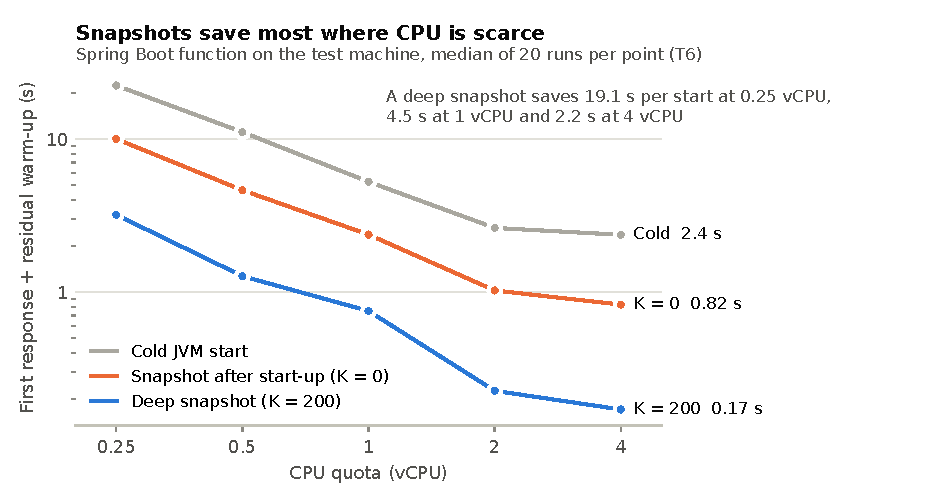
\includegraphics[width=\textwidth]{fig9_cliff}}%
  {\fbox{\parbox{0.9\textwidth}{\centering figures/fig9\_cliff.pdf not rendered yet:
  run \texttt{python3 figures/make\_figures.py}}}}
\caption{Time to first response plus residual warm-up against the CPU quota, for a cold start, a
snapshot after start-up ($K = 0$) and a deep snapshot ($K = 200$); median of 20 runs per point,
logarithmic axes.}
\label{fig:m-cliff}
\end{figure}

\section{Safety: what restored copies share}
\label{sec:m-uniq}

Copies restored from one image start with the same memory~\cite{brooker2021}. Ten copies were
restored from one image and each reported hashes of values it had created at start-up. Without
reset hooks, a \texttt{java.util.Random}, a secret token generated at start-up (even from a
\texttt{SecureRandom}) and \texttt{Math.random()} returned the same value in all ten copies; the
JDK's own \texttt{SecureRandom} and \texttt{UUID} sources were re-seeded on restore and differed.
A CRaC resource hook that re-seeds the \texttt{Random} and regenerates the token fixed those two
(ten distinct values), but \textbf{not \texttt{Math.random()}}, whose generator is private to the
JDK and has no re-seed interface. A snapshot builder must therefore either refuse functions that
call \texttt{Math.random()} before the checkpoint, or reset its generator by reflection; this is
one concrete reason why not every function is safe to snapshot.

\section{What the measurements change}
\label{sec:m-changes}

\begin{itemize}
\item \textbf{The model's inputs.} Restore time $r$: 74--84\,ms at 1\,vCPU and 282--375\,ms at
      0.25\,vCPU for a deep snapshot (was 650\,ms). Contention $\beta \approx 0.05$ into existing
      containers (was an assumption). Residual warm-up after a restore: 720\,ms over 200 requests
      at $K = 50$, 1\,vCPU (was 63\,ms). Start-up cap: about two cores (was one).
\item \textbf{The weight shifts from timing to depth and CPU.} With $r \approx 80$\,ms, restoring
      ahead hides about 80\,ms per stage at 1\,vCPU and about 300\,ms at 0.25\,vCPU. The residual
      warm-up and the CPU a start-up gets now matter more than when it starts.
\item \textbf{The design.} Restore into existing containers; keep images in memory; boost a
      start-up until its warm-up is done; keep re-warming; choose the depth from the residual
      curve rather than from a compile counter that has not levelled off; exclude or patch
      functions that use \texttt{Math.random()} before the checkpoint.
\end{itemize}

\begin{table}[htbp]
\centering
\caption{Registered predictions and outcomes.}
\label{tab:m-predictions}
\small
\begin{tabular}{@{}p{0.5\textwidth}p{0.42\textwidth}@{}}
\toprule
prediction & outcome \\
\midrule
a deep snapshot reaches the first response $\ge 5\times$ sooner than the AOT cache & confirmed, 25--30$\times$ \\
residual warm-up after a deep restore $\ll$ after the AOT cache & falsified: similar \\
CRIU a few hundred ms slower than Warp & falsified: 17--91\,ms \\
$\beta < 0.3$ for $N \le 4$ & confirmed into existing containers; through \texttt{docker run} only at 0.25\,vCPU \\
Docker's own part of $\beta$: 0.1--0.3 & falsified: 0.6--0.8 \\
image size flat in $K$ & confirmed, 82--88\,MB \\
residual warm-up $\approx 63$\,ms at $K = 50$, levelling off & falsified: 720\,ms, still falling at $K = 200$ \\
restore from disk $< 50$\,ms slower than from memory & falsified: 440--810\,ms \\
$L(K) > 0$, larger at low CPU; re-warming recovers $\ge 30\%$ & confirmed; recovers more than all of it \\
reset hooks make every value distinct & falsified for \texttt{Math.random()} \\
cold warm-up cliff 13--35$\times$ & falsified in size: $10.3\times$ \\
deep snapshots flatten the cliff (ratio $< 5\times$) & falsified as a ratio ($20.6\times$); holds in absolute time \\
start-up $\approx 4\times$ faster from 0.25 to 1\,vCPU at the same CPU-seconds & confirmed ($3.5$--$4.5\times$); continues to 2 cores \\
boosted start-ups serve later requests as fast & confirmed for deep restores; falsified for cold starts and $K = 0$ \\
\bottomrule
\end{tabular}
\end{table}

\section{Threats to validity}
\label{sec:m-threats}

\begin{itemize}
\item \textbf{One function.} All numbers are for one Spring Boot function. The residual warm-up and
      the depth at which it levels off depend on the function; the qualitative results
      (snapshot vs AOT cache, contention into existing containers, the shape of the speed-up)
      are the ones to generalise, and the next experiments add Python and ML stages.
\item \textbf{A virtual machine.} The host is VMware with no measured steal time; the disk is
      virtual, so the disk tier's cost is specific to it.
\item \textbf{Memory was not measured.} The cgroup's memory counter included the page cache it
      had accumulated, so the processes' own memory is unknown; image sizes are reported instead.
\item \textbf{The bimodal restores} (\cref{sec:m-depth}) are unexplained.
\item \textbf{Privileges.} Containers ran with \texttt{--privileged}; the minimal capability set,
      and CRIU inside pre-created containers, are left to the OpenWhisk integration.
\end{itemize}

\bibliographystyle{plain}
\bibliography{theory}
\end{document}
